\documentclass{article}
\usepackage[utf8]{inputenc}
\usepackage[spanish]{babel}
\usepackage{amsthm}
\usepackage{amssymb}
\usepackage{amsmath}
\usepackage{fancyhdr}
\usepackage{graphicx}
\usepackage[dvipsnames, table]{xcolor}
\usepackage[framemethod=tikz]{mdframed}
\usepackage{multicol}
\usepackage{tabularx}
\usepackage{pifont}
\setlength{\tabcolsep}{3pt}
\decimalpoint
\newcommand{\xmark}{\ding{55}}
\definecolor{mycolor}{rgb}{0.122, 0.435, 0.698}

\newmdenv[innerlinewidth=0.5pt, roundcorner=4pt,linecolor=mycolor,innerleftmargin=6pt,
innerrightmargin=6pt,innertopmargin=6pt,innerbottommargin=6pt]{mybox}


\setlength\parindent{0pt}

\newtheorem{definition}{Definición}
\newtheorem{proposition}{Proposición}

\renewcommand{\headrulewidth}{0.4pt}

\begin{document}
\date{13 - 20 marzo de 2020}
\title{ \textbf{Topología} \\
Semana 2: Conjuntos cerrados, puntos límite y espacios de Hausdorff}
%\author{Docente: Gabriel Chicas Reyes, MSc.\\ 
	%			Alumno: Kevin López Aquino }
\maketitle	
\begin{mybox}
	\textbf{1.} Sea $X$ un conjunto y $\mathcal{C} \subseteq \mathcal{P}(X)$. Supongamos que $\varnothing, X \in \mathcal{C}$ y que las intersecciones arbitrarias y uniones finitas de elementos de $\mathcal{C}$ están en $\mathcal{C}$. Entonces, 
	$$ \mathcal{T} = \{ X \backslash C \mid C \in \mathcal{C} \} $$ 
	es una topología sobre $X$.
\end{mybox}	 
\begin{proof}
Primero notamos que $\varnothing$ y $X$ están en $\mathcal{T}$. Consideremos una colección $\{ X \backslash C_{i} \}_{i \in J}$ no vacía de elementos de $\mathcal{C}$. Entonces, 
$$ \bigcup _{i \in J} \left( X \backslash C_{i} \right)  = X \backslash \bigcap_{i \in J} C_{i} \in \mathcal{T}.$$
Además, si tomamos dos elementos $X\backslash C_{1}, X\backslash C_{2}$ de $\mathcal{T}$,
$$ (X \backslash C_{1}) \cap (X \backslash C_{2}) = X \backslash \left( C_{1} \cup C_{2} \right) \in \mathcal{T}. $$
\end{proof}

La demostración anterior nos dice que podríamos tomar las propiedades de los conjuntos cerrados como punto de partida y luego demostrar las propiedades de los conjuntos abiertos enunciadas en la definición usual de una topología. \\

\begin{mybox}
	\textbf{2. } Si $A$ es cerrado en $Y$ y $Y$ es cerrado en $X$, $A$ es cerrado en $X$.
\end{mybox}	
\begin{proof}
Podemos escribir $A = C \cap Y$, donde $C$ es cerrado en $X$. Al ser la intersección de dos conjuntos cerrados en $X$, $A$ es cerrado en $X$. 
\end{proof}
\begin{mybox}
	\textbf{3. } Sean $X$ y $Y$ espacios topológicos. Si $A$ es cerrado en $X$ y $B$ es cerrado en $Y$, $A \times B$ es cerrado en $X \times Y$. 
\end{mybox}	
\begin{proof}
	Notamos que $X \backslash A$ es abierto en $X$ y $Y \backslash B$ es abierto en $Y$. Notamos que 
	$$ \left( X \times Y \right) \backslash \left( A \times B \right) =   \left( \left( X \backslash A \right) \times Y \right) \cup \left( X \times \left( Y \backslash B \right) \right). $$
	El lado derecho es la unión de conjuntos abiertos en $X \times Y$, lo que implica que $A \times B$ es cerrado.  
\end{proof}

\begin{mybox}
\textbf{4. } 	Si $U$ es abierto en $X$ y $A$ es cerrado en $X$, entonces $U \backslash A$ es abierto y $A \backslash U$ es cerrado.
\end{mybox}
\begin{proof}
	Notamos que 
	$$ X \backslash ( U \backslash  A) = (X \backslash U) \cup A $$
	es la unión de dos conjuntos cerrados y es, por tanto, cerrado. Concluimos que $U\backslash A$ es abierto.  De forma similar,
	$$X \backslash ( A \backslash  U) = (X \backslash A) \cup U $$
	es la unión de dos conjuntos abiertos, de lo que se sigue que su complemento, $A \backslash U$, es cerrado. 
\end{proof}	

\begin{mybox}
	\textbf{5. } Sea $X$ un conjunto ordenado, dotado de la topología del orden. Entonces, 
	$$ \text{cl}(a, b) \subseteq [a, b ] $$. 
\end{mybox}	
\begin{proof}
	Notamos que $[a, b]$ es un conjunto cerrado y que $(a, b) \subseteq [a, b]$. Se sigue que $\text{cl}(a, b) \subseteq [a, b]$.
\end{proof}

Además, si $a$ no tiene sucesor inmediato, podemos afirmar que $a \in \text{cl}(a, b)$. De manera similar, si $b$ no tiene predecesor inmediato, podemos afirmar que $b \in \text{cl}(a, b)$, de forma que $\text{cl}(a, b) = [a, b]$. Si no nos limitamos a puntos $a$ y $b$ específicos, tenemos el siguiente resultado. \\

\textbf{Proposición. } Sea $(X, \leq )$ un conjunto ordenado. Si la relación de orden sobre $X$ es densa, para cualesquiera $a$ y $b$ tales que $a < b$ tenemos que $\text{cl}(a, b) = [a, b]$.
\begin{proof}
	Antes mostramos que $\text{cl}(a, b) \subseteq [a, b]$. Notamos que si el orden es denso, todo entorno de $a$ debe intersecar a $(a, b)$. De forma similar, todo entorno de $b$ debe intersecar a $(a, b)$. Se sigue que $\text{cl}(a, b) = [a, b]$.
\end{proof}

\begin{mybox}
	\textbf{6.} Sean $A, B$ y $A_{\alpha}$ subconjuntos de un espacio topológico $X$. Entonces, se cumplen las siguientes proposiciones: \\
	
	\textbf{(a)} Si $A\subseteq B$, $\text{cl}(A) \subseteq \text{cl}(B)$.  \\
	
    \textbf{(b)} $\text{cl}(A) \cup \text{cl}(B) = \text{cl}(A \cup B) .$ \\
    
    \textbf{(c)} $\bigcup_{\alpha \in J} \text{cl}(A_{\alpha}) \subseteq  \text{cl}\left( \bigcup_{\alpha \in J} A_{\alpha} \right)$.  
	
\end{mybox}	
$\textbf{(a)}$ Notamos que $A \subseteq \text{cl}(B)$.

\begin{mybox}
	\textbf{9. }Sean $A \subseteq X, B \subseteq Y$. En el espacio $X \times Y$,
	$$ \text{cl}(A \times B) = \text{cl}(A) \times \text{cl}(B) .$$
\end{mybox}	
\begin{proof}
	Notamos que $\text{cl}(A) \times \text{cl}(B)$ es cerrado en $A \times B$. Además, $A \times B \subseteq \text{cl}(A) \times \text{cl}(B)$. Esto implica que $\text{cl}(A \times B) \subseteq \text{cl}(A) \times \text{cl}(B)$.\\
	Por otro lado, consideremos un punto $(x, y) \in \text{cl}(A) \times \text{cl}(B)$. Entonces, cualquier básico $U \times V$ que contenga a $(x, y)$ interseca a $A \times B$, lo que implica que $(x, y) \in \text{cl}(A \times B)$. Así, $\text{cl}(A) \times \text{cl}(B) \subseteq \text{cl}(A \times B). $ 
\end{proof}

\begin{mybox}
	\textbf{10. } Todo espacio dotado de la topología del orden es de Hausdorff. 
\end{mybox}	
\begin{proof}
	Consideremos $x, y \in X$ y supongamos, sin pérdida de generalidad, que $x < y$. Analizamos dos casos. \\
	\textit{Caso I. } Existe un $z$ que verifica $x < z < y$. Entonces $x$ está en $(- \infty, z)$ y $y$ está en  $(z, \infty)$. Ambos rayos son conjuntos abiertos y disjuntos. \\
	\textit{Caso II. } Si $y$ es sucesor inmediato de $x$, tenemos que $x \in ( - \infty, y) = (- \infty,x]$ y $y \in (x, \infty) = [y, \infty)$. De igual forma, ambos conjuntos son abiertos y disjuntos. \\
	Así, en cada caso podemos encontrar entornos disjuntos de $x$ y $y$, de lo que se sigue que $X$ es un espacio de Hausdorff. 
\end{proof}

\begin{mybox}
\textbf{11. } Muestre que el producto de dos espacios de Hausdorff es Hausdorff. 	
\end{mybox}	
\begin{proof}
	Sean $X$ y $Y$ dos espacios de Hausdorff. Tomemos dos puntos $(x_{1}, y_{1}), (x_{2}, y_{2})$ distintos de $X \times Y$. Entonces, $x_{1} \neq x_{2}$ o $y_{1} \neq y_{2}$. Supongamos, sin pérdida de generalidad, que $x_{1} \neq x_{2}$. Puesto que $X$ es Hausdorff, podemos elegir entornos disjuntos $U_{1}, U_{2} \subseteq X$ de $x_{1}$ y $x_{2}$, respectivamente.  Entonces, $U_{1} \times Y$ y $(x_{2}, y_{2})$ son entornos de $(x_{1}, y_{1})$ y $U_{2} \times Y$, respectivamente, en la topología producto sobre $X \times Y$. Además, 
	$$ \left( U_{1} \times Y \right) \cap \left( U_{2} \times Y \right) =   \left( U_{1} \cap U_{2} \right) \times Y = \varnothing, $$
	con lo que queda demostrada la proposición. 
\end{proof}

\begin{mybox}
	\textbf{12. } Demuestre que un subespacio de Hausdorff es Hausdorff. 
\end{mybox}	
\begin{proof}
	Sea $X$ un espacio de Hausdorff y $Y$ un subespacio de este. Consideremos dos puntos distintos $x$ y $y$ en $Y$. Entonces, podemos encontrar abiertos $U, V$ de $X$ que contengan a $x$ y a $y$, respectivamente, y sean disjuntos. Se sigue que $Y \cap U$ y $Y \cap V$ son entornos de $x$ y de $y$, respectivamente, en el subespacio $Y$. Además, son entornos disjuntos: $(Y \cap U) \cap (Y \cap V) = Y \cap U \cap V = \varnothing.$
\end{proof}

\begin{mybox}
	\textbf{13. } Muestre que $X$ es Hausdorff si y solo si la \textbf{diagonal}
	$$ \Delta = \{ (x, x) \mid x \in X \} $$
	es cerrada en $ X \times X$.
\end{mybox}	
\begin{proof}
	$(\Leftarrow)$ Supongamos que $\Delta$ es cerrada en $X \times X$. Entonces, 
	$$ \left( X \times X \right)  \backslash \Delta = \{ (x, y) \in X \times X \mid x \neq y \}$$ 
es abierto en $X \times X$. Esto implica que para cualesquiera $x, y \in X$ tales que $x \neq y$, existen abiertos $U, V \subseteq X$ tales que
$$ (x, y) \in U \times V \subseteq  \left( X \times X \right)  \backslash \Delta. $$
De lo anterior se observa que no puede existir un elemento en $U \cap V$. Así, para $x$ y $y$ de $X$ distintos, hemos construido entornos disjuntos. Se sigue que $X$ es Hausdorff.\\
$(\Rightarrow)$ Ahora supongamos que $X$ es Hausdorff. Mostramos que $\left( X \times X \right)  \backslash \Delta$ es abierto. Si $(x, y) \in \left( X \times X \right)  \backslash \Delta$, deducimos que $x \neq y$ y que existen entornos disjuntos $U, V$ de $x$ y $y$, respectivamente. Notamos que $ (U \times V) \cap \Delta = \varnothing$, de forma que 
$$(x, y) \in U \times V \subseteq \left( X \times X \right)  \backslash \Delta.$$ 
Así, para cada punto en $\left( X \times X \right)  \backslash \Delta$ podemos encontrar un elemento básico dentro de este conjunto que lo contiene, de lo que se sique que $\left( X \times X \right)  \backslash \Delta$ es abierto. 
\end{proof}

\begin{mybox}
	\textbf{14. } En la topología cofinita sobre $\mathbb{R}$, la sucesión $x_{n} = 1/n$ converge a todo número real. 
\end{mybox}	
\begin{proof}
	Consideremos un número real $r$ y un entorno $U$ de este. Entonces, el conjunto $U$ contiene todos los números reales salvo una cantidad finita de ellos. Se sigue que debe existir un número natural $N$ a partir del cual todos los números de la forma $1/n$, con $n \geq N$, estén en $U$.  
\end{proof}

\begin{mybox}
	\textbf{15. } Pruebe que el axioma $T_{1}$ es equivalente a la condición que para cada par de puntos distintos de $X$, cada uno posee un entorno que no contiene al otro. 
\end{mybox}	
\begin{proof}
	$(\Leftarrow)$ Supongamos que para par de puntos distintos de un espacio $X$, cada uno tiene un entorno que no contiene al otro. Demostraremos que todos los conjuntos unipuntuales son cerrados en $X$, de lo que se sigue que cualquier conjunto finito también será cerrado. \\
	Sea $x$ un punto de $X$. Mostramos que $\text{cl}\{x\} = \{x\}$. Consideremos un puntuo $y \neq x$. Por la hipótesis, podemos encontrar un entorno $V$ de $y$ tal que $x \notin V$; es decir, $V \cap \{x\} = \varnothing$. Así, hemos construido un entorno de $y$ que no interseca a $\{ x \}$, de lo que se sigue que $y \notin \text{cl}\{x\}$. Por tanto, $\text{cl}\{x\} = \{x\}$. \\
	$(\Rightarrow)$ Ahora supongamos que los subconjuntos finitos de $X$ son cerrados y tomemos dos puntos distintos $x$ y $y$ de $X$. Entonces, el conjunto $X \backslash \{y\}$ es un entorno de $x$ que no contiene a $y$. De manera similar, $X \backslash \{ x \}$ es un entorno de $y$ que no contiene a $x$.
\end{proof}
La parte $(\Leftarrow)$ sigue el mismo argumento de la demostración del \textbf{teorema 17.8} de \textbf{[1]}. Este hecho ilustra que no necesitamos algo tan fuerte como la propiedad de Hausdorff para que los conjuntos finitos sean cerrados: basta con una propiedad más débil como el axioma $T_{1}$. 
\vspace{0.5cm}
\begin{mybox}
	\textbf{17. } Considere el espacio $\mathbb{R}_{\ell}$ y la topología sobre $\mathbb{R}$ generada por la base
	$$ \mathcal{C} = \{ [p, q) \mid p < q \hspace{0.2cm} \text{y} \hspace{0.2cm} p, q \in \mathbb{Q} \} .$$
	Determine las clausuras de los intervalos $A = (0, \sqrt{2})$ y $B = (\sqrt{2}, 3)$ en estas dos topologías. 
\end{mybox}	
$\bullet$ Consideremos la clausura de $(0, \sqrt{2})$ en $\mathbb{R}_{\ell}$. Notamos que los intervalos $(a, b)$ son abiertos en esta topología, pero no son cerrados. Esto se puede observar al tomar el complemento
$$ \mathbb{R} \backslash (a, b) = (- \infty, a] \cup [b, \infty). $$
Entonces, no existe un intervalo semiabierto que contenga a $a$ y a la vez esté contenido en este conjunto. Por otro lado, los conjuntos $[a, b)$ son tanto cerrados como abiertos. Así, decimos que 
$$ \text{cl}(0, \sqrt{2}) = [0, \sqrt{2}). $$
Notamos que $0$ está en la clausura de $(0, \sqrt{2})$, porque todo intervalo semiabierto que contenga a $0$ interseca este conjunto. Por otro lado, si $x$ es un número real tal que $x < 0$, el elemento básico $[x, 0)$ no interseca a $(0, \sqrt{2})$. De igual forma, si $x \geq \sqrt{2}$, $[\sqrt{2}, \infty)$ es un entorno de $x$ que no interseca a $(0, \sqrt{2})$. \\

$\bullet$ Ahora consideremos la clausura de $(0, \sqrt{2})$ en $\mathbb{R}$ equipado con $\mathcal{T_{C}}$. Notamos que $0$ está en la clausura, dado que todo básico $[p, q)$ que contenga a $0$ interseca a $(0, \sqrt{2})$. De forma más interesante, $\sqrt{2}$ está incluido en la clausura de $(0, \sqrt{2})$. Esto se sigue del hecho que en todo básico $[p, q)$ que contenga a $\sqrt{2}$, el extremo izquierdo $p$ siempre es menor que $\sqrt{2}$. Por otro lado, si $x < 0$, el elemento básico $[p, 0)$, donde $p \leq x$ es racional, no interseca a $(0, \sqrt{2})$. Si $x > \sqrt{2}$, $(\sqrt{2}, \infty)$ es un entorno de $x$ que no interseca a $(0, \sqrt{2})$. Así, $\text{cl}(0, \sqrt{2}) = [0, \sqrt{2}]$. \\

$\bullet$ En ambos espacios topológicos, se tiene que $\text{cl}(\sqrt{2}, 3) = [\sqrt{2}, 3)$. Notemos que en cualquiera de las topologías, si un elemento básico contiene a $\sqrt{2}$, siempre intersecará $(\sqrt{2}, 3)$. Por otro lado, si $x < \sqrt{2}$, siempre podemos encontrar un entorno de $x$ en ambas topologías que no interseque este conjunto. Lo mismo si $x \geq 3$.  \hspace*{\fill} $\blacksquare$
\vspace{0.5cm}

\begin{figure}[h]
	\centering 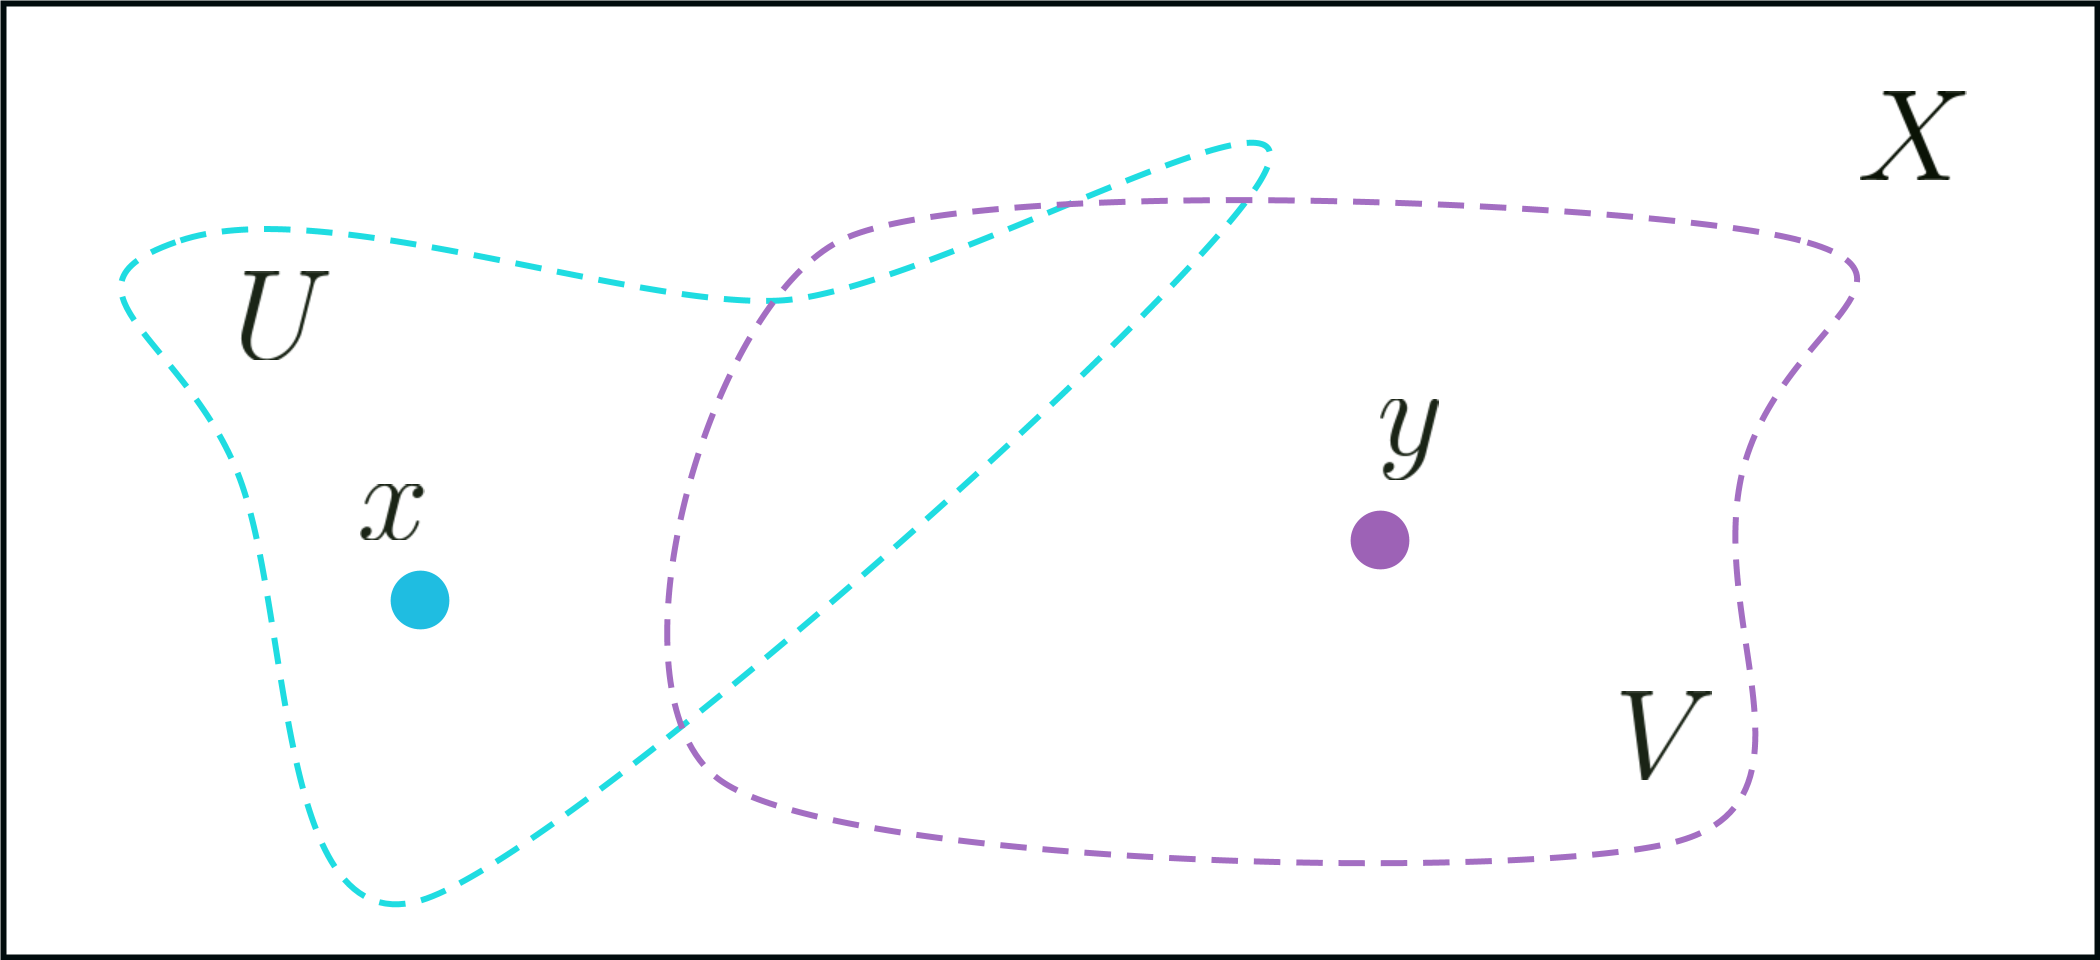
\includegraphics[scale=0.15]{e2fig.png}
	\caption{En un espacio $X$ que cumple el axioma $T_{1}$ siempre podemos hacer lo mostrado en la figura, pero no podemos garantizar que los entornos sean disjuntos, a diferencia de un espacio de Hausdorff. }
\end{figure}

\begin{mybox}
	\textbf{19. } Si $A \subseteq X$, definimos la \textbf{frontera} de $A$ mediante la ecuación
	$$ \partial A = \text{cl}(A) \cap \text{cl}(X \backslash A). $$
	\textbf{(a)} Pruebe que $\text{int}(A)$ y $\partial A$ son disjuntos y que $\text{cl}(A) = \text{int}(A) \cup \partial A$. \\
	
	\textbf{(b)} Muestre que $\partial A = \varnothing $ si y solo si $A$ es abierto y cerrado a la vez. \\
	
	\textbf{(c)} Muestre que $U$ es abierto si y solo si $\partial U = \text{cl}(U) \backslash U$.\\
	
	\textbf{(d)} Si $U$ es abierto, ¿es cierto que $U = \text{int}(\text{cl}(U))$?
\end{mybox}	
$\bullet$ Para ver que el interior de $A$ y su frontera son disjuntos, suponemos que existe un punto $x$ en ambos conjuntos. Al estar en el interior de $A$, se sigue que existe un $U$ entorno de $x$ contenido en $A$. Sin embargo, $x \in \text{cl}(X \backslash A)$, lo que implica que $U$ debe intersecar a $X \backslash A$. Teniendo en cuenta que $U \subseteq A$, esto resulta imposible. \\

Para demostrar que al unir el interior de un conjunto $A$ con su frontera obtenemos su clausura, primero notamos que la definición implica que $\partial A \subseteq \text{cl}(A)$. Además, sabemos que $\text{int}(A) \subseteq \text{cl}(A)$, de forma que $\text{int}(A) \cup \partial A \subseteq \text{cl}(A)$.\\
Para demostrar que $\text{cl}(A) \subseteq \text{int}(A) \cup \partial A$, supongamos que $x$ está en $\text{cl}(A)$ y no está en $\text{int}(A)$, con el fin de mostrar que $x \in \partial A$. Si tomamos un entorno arbitrario de $x$, notamos que no puede estar contenido en $A$, de forma que se debe intersecar con $X \backslash A$. Así, $x \in \text{cl}(X \backslash A)$, de lo que se sigue la conclusión. $\hspace*{\fill} \blacksquare$ \\

$\bullet \hspace{0.2cm} (\Leftarrow)$ Supongamos que $A$ es abierto y cerrado a la vez. Entonces, podemos decir lo mismo de $X \backslash A$. Usando el hecho que ambos conjuntos son cerrados, inferimos que 
$$ \text{cl}(X \backslash A) = X \backslash A \hspace{0.2cm} \text{y} \hspace{0.2cm} \text{cl}(A) = A.$$
Así, $ \partial A = A \cap (X \backslash A) = \varnothing.$   \\
$(\Rightarrow)$ Ahora supongamos que $\partial A = \varnothing.$ Por la parte $\textbf{(a)}$, se sigue que $\text{int} (A) = \text{cl}(A)$. En vista que $\text{int}(A) \subseteq A \subseteq \text{cl}(A)$, podemos deducir que $A = \text{int}(A) = \text{cl}(A)$, de forma que $A$ es abierto y cerrado. $\hspace*{\fill} \blacksquare$ \\

\begin{figure}[h]
	\centering 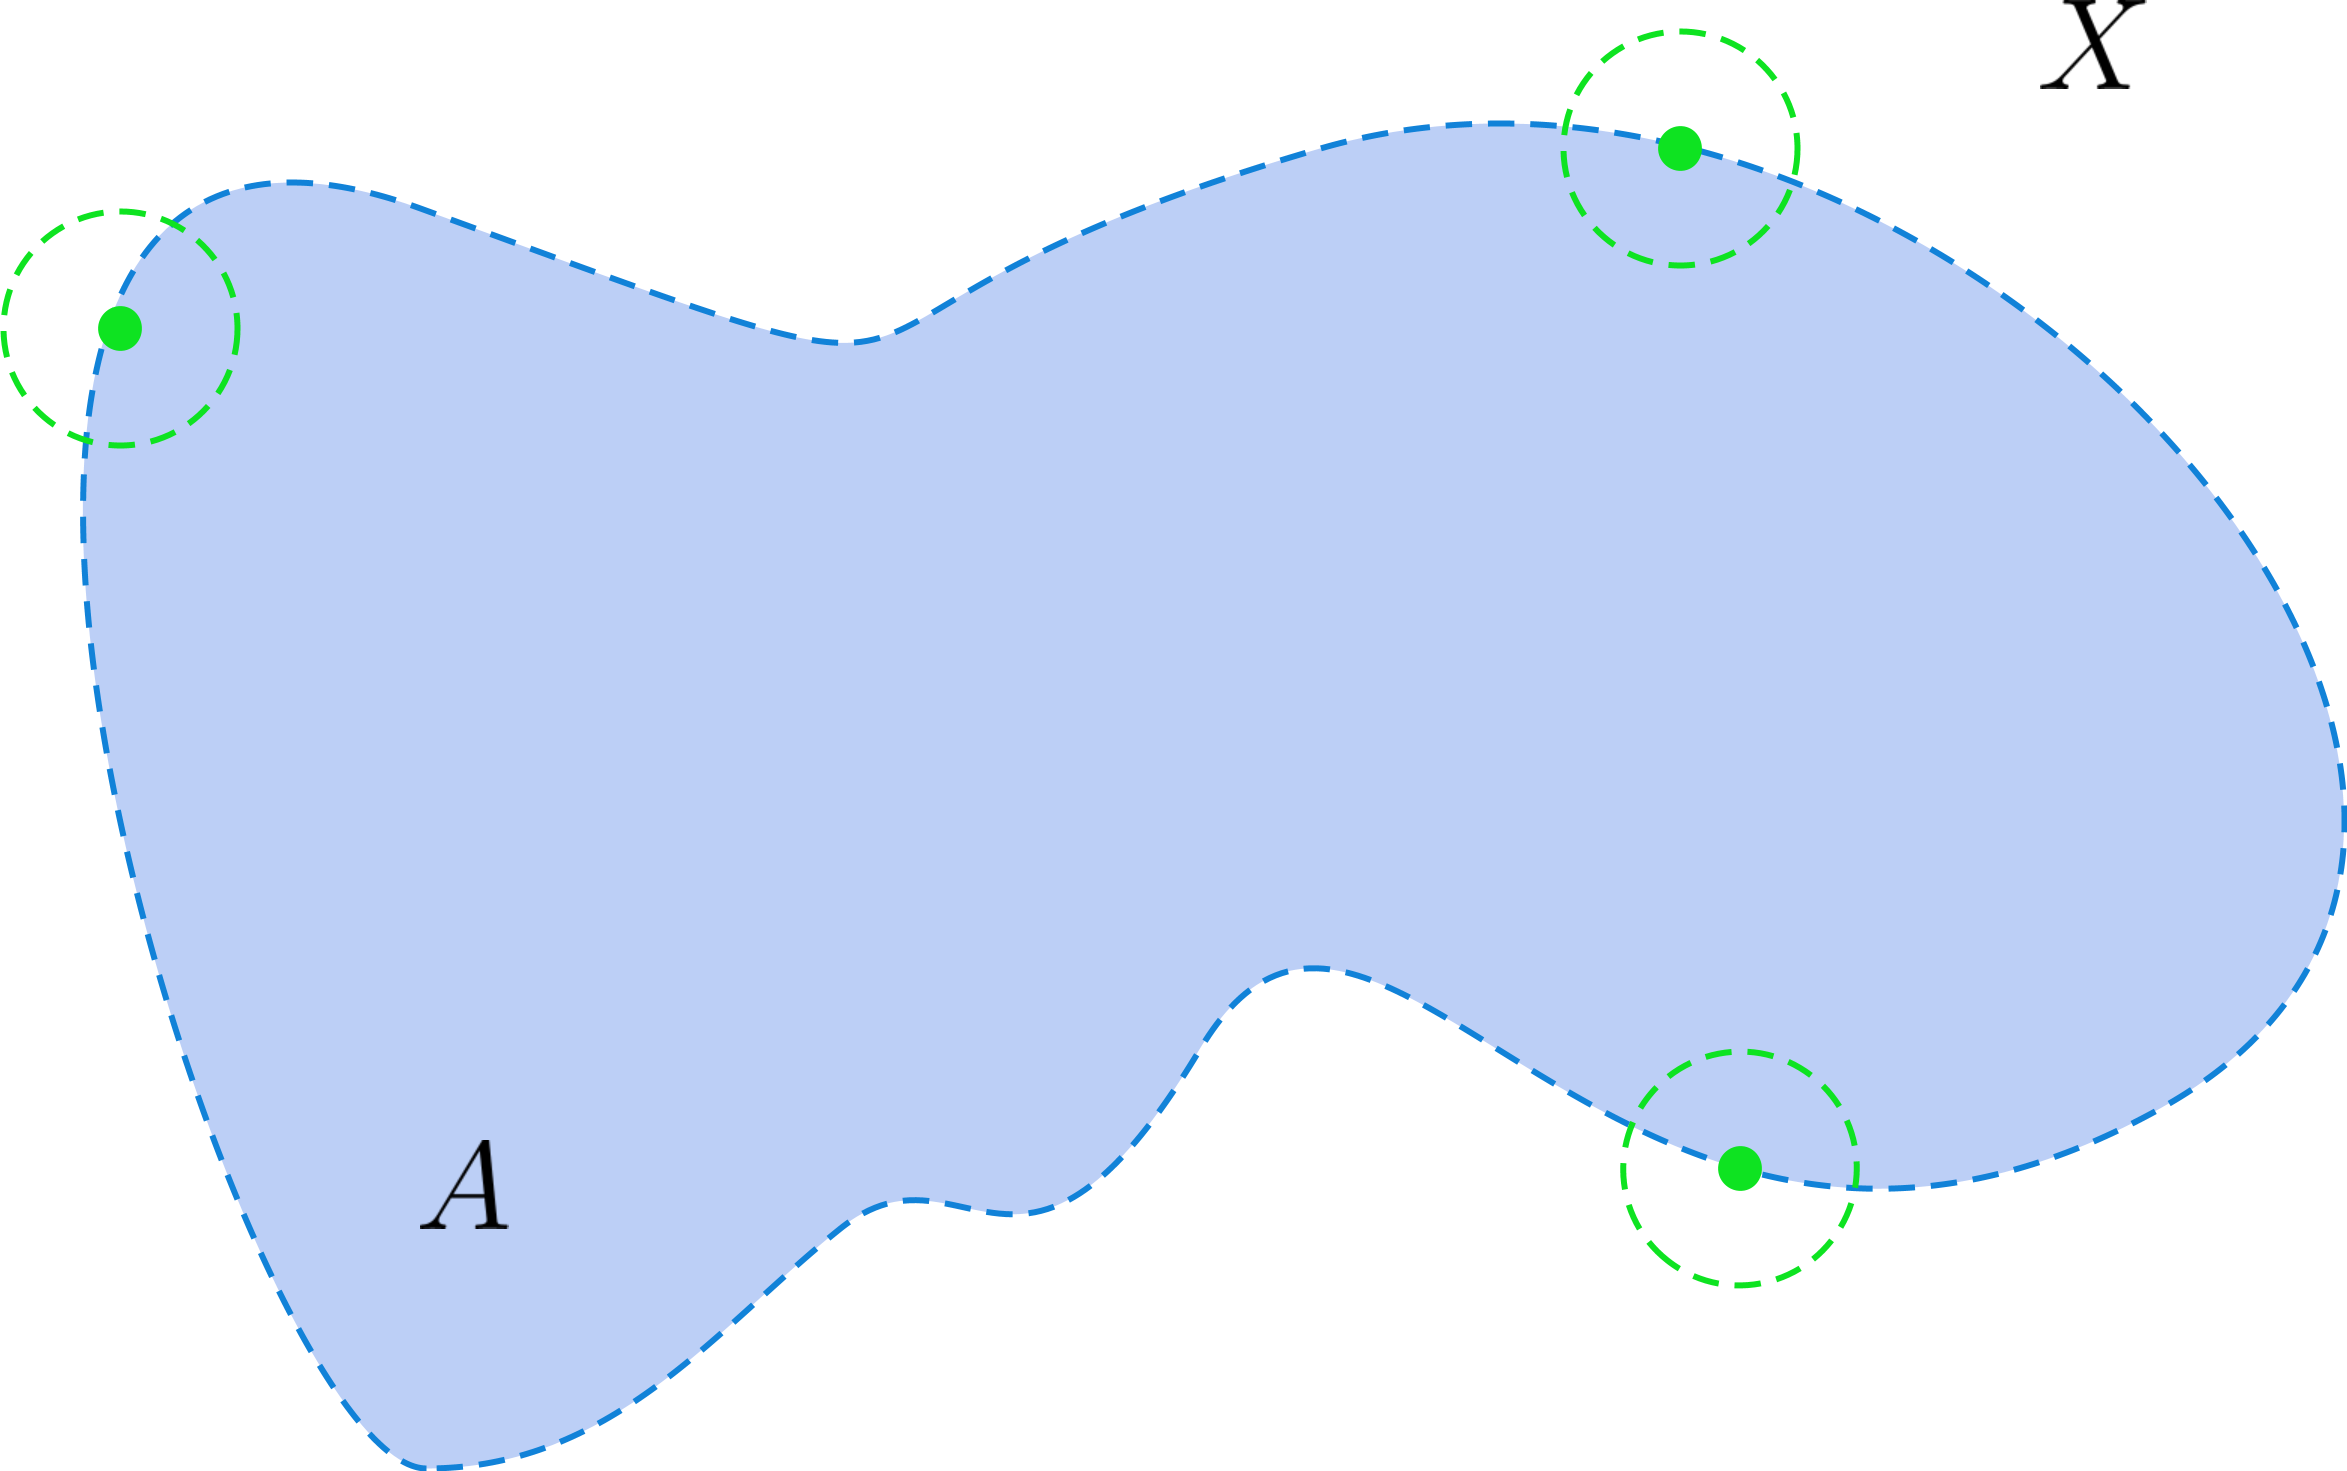
\includegraphics[scale=0.13]{e2fig2.png}
	\caption{Si un punto está en la frontera de $A$, cada entorno de ese punto contiene puntos dentro de $A$ y fuera de $A$. }
\end{figure}

$\bullet \hspace{0.2cm}  (\Rightarrow)$ Supongamos que $U$ es abierto. Entonces, $U = \text{int}(U)$. Esto, junto con la parte $\textbf{(a)}$ implica que $\text{cl}(U) = \text{int}(U) \cup \partial U = U \cup \partial U$.  Además, sabemos que $\text{int}(U) = U$ y $\partial U$ son disjuntos, de forma que al remover los elementos de $U$ de $\text{cl}(U)$ solo quedarán los puntos en la frontera: $\text{cl}(U) \backslash U = \partial U$. \\
$(\Leftarrow)$ Ahora supongamos que $\text{cl}(U) \backslash U = \partial U$. Procedemos por contradicción, suponiendo que $U$ es no abierto. Esto implica que existe un punto $x$ en $U$ tal que ninguno de sus entornos está contenido en $U$. De forma equivalente, podemos decir que cualquier entorno de $x$ interseca a $X \backslash U$. Así, $x \in \text{cl}(X \backslash U)$. Además, $x \in \text{cl}(U)$, lo que implica que $x \in \partial U$. Por la suposición inicial, podemos deducir que $x \notin U$, lo cual es absurdo. $\hspace*{\fill} \blacksquare$ \\

\newpage

$\bullet$ No. El conjunto $U = (1, 2) \cup (2, 3)$ es abierto en la topología usual sobre $\mathbb{R}$, pero $\text{int}(\text{cl}(U)) = (1, 3) \neq U.$\\

\textbf{Definición. } Sea $X$ un espacio topológico y $U \subseteq X$. Decimos que $U$ es \textbf{abierto regular} si $\text{int}(\text{cl}(U)) = U$. \\

El ejemplo anterior muestra que no todos los conjuntos abiertos son abiertos regulares. De la definición notamos que al ser el interior de otro conjunto, todos los regulares abiertos son abiertos. ¿Qué sucede con el ejemplo $U$ presentado anteriormente?

\begin{figure}[h]
	\centering 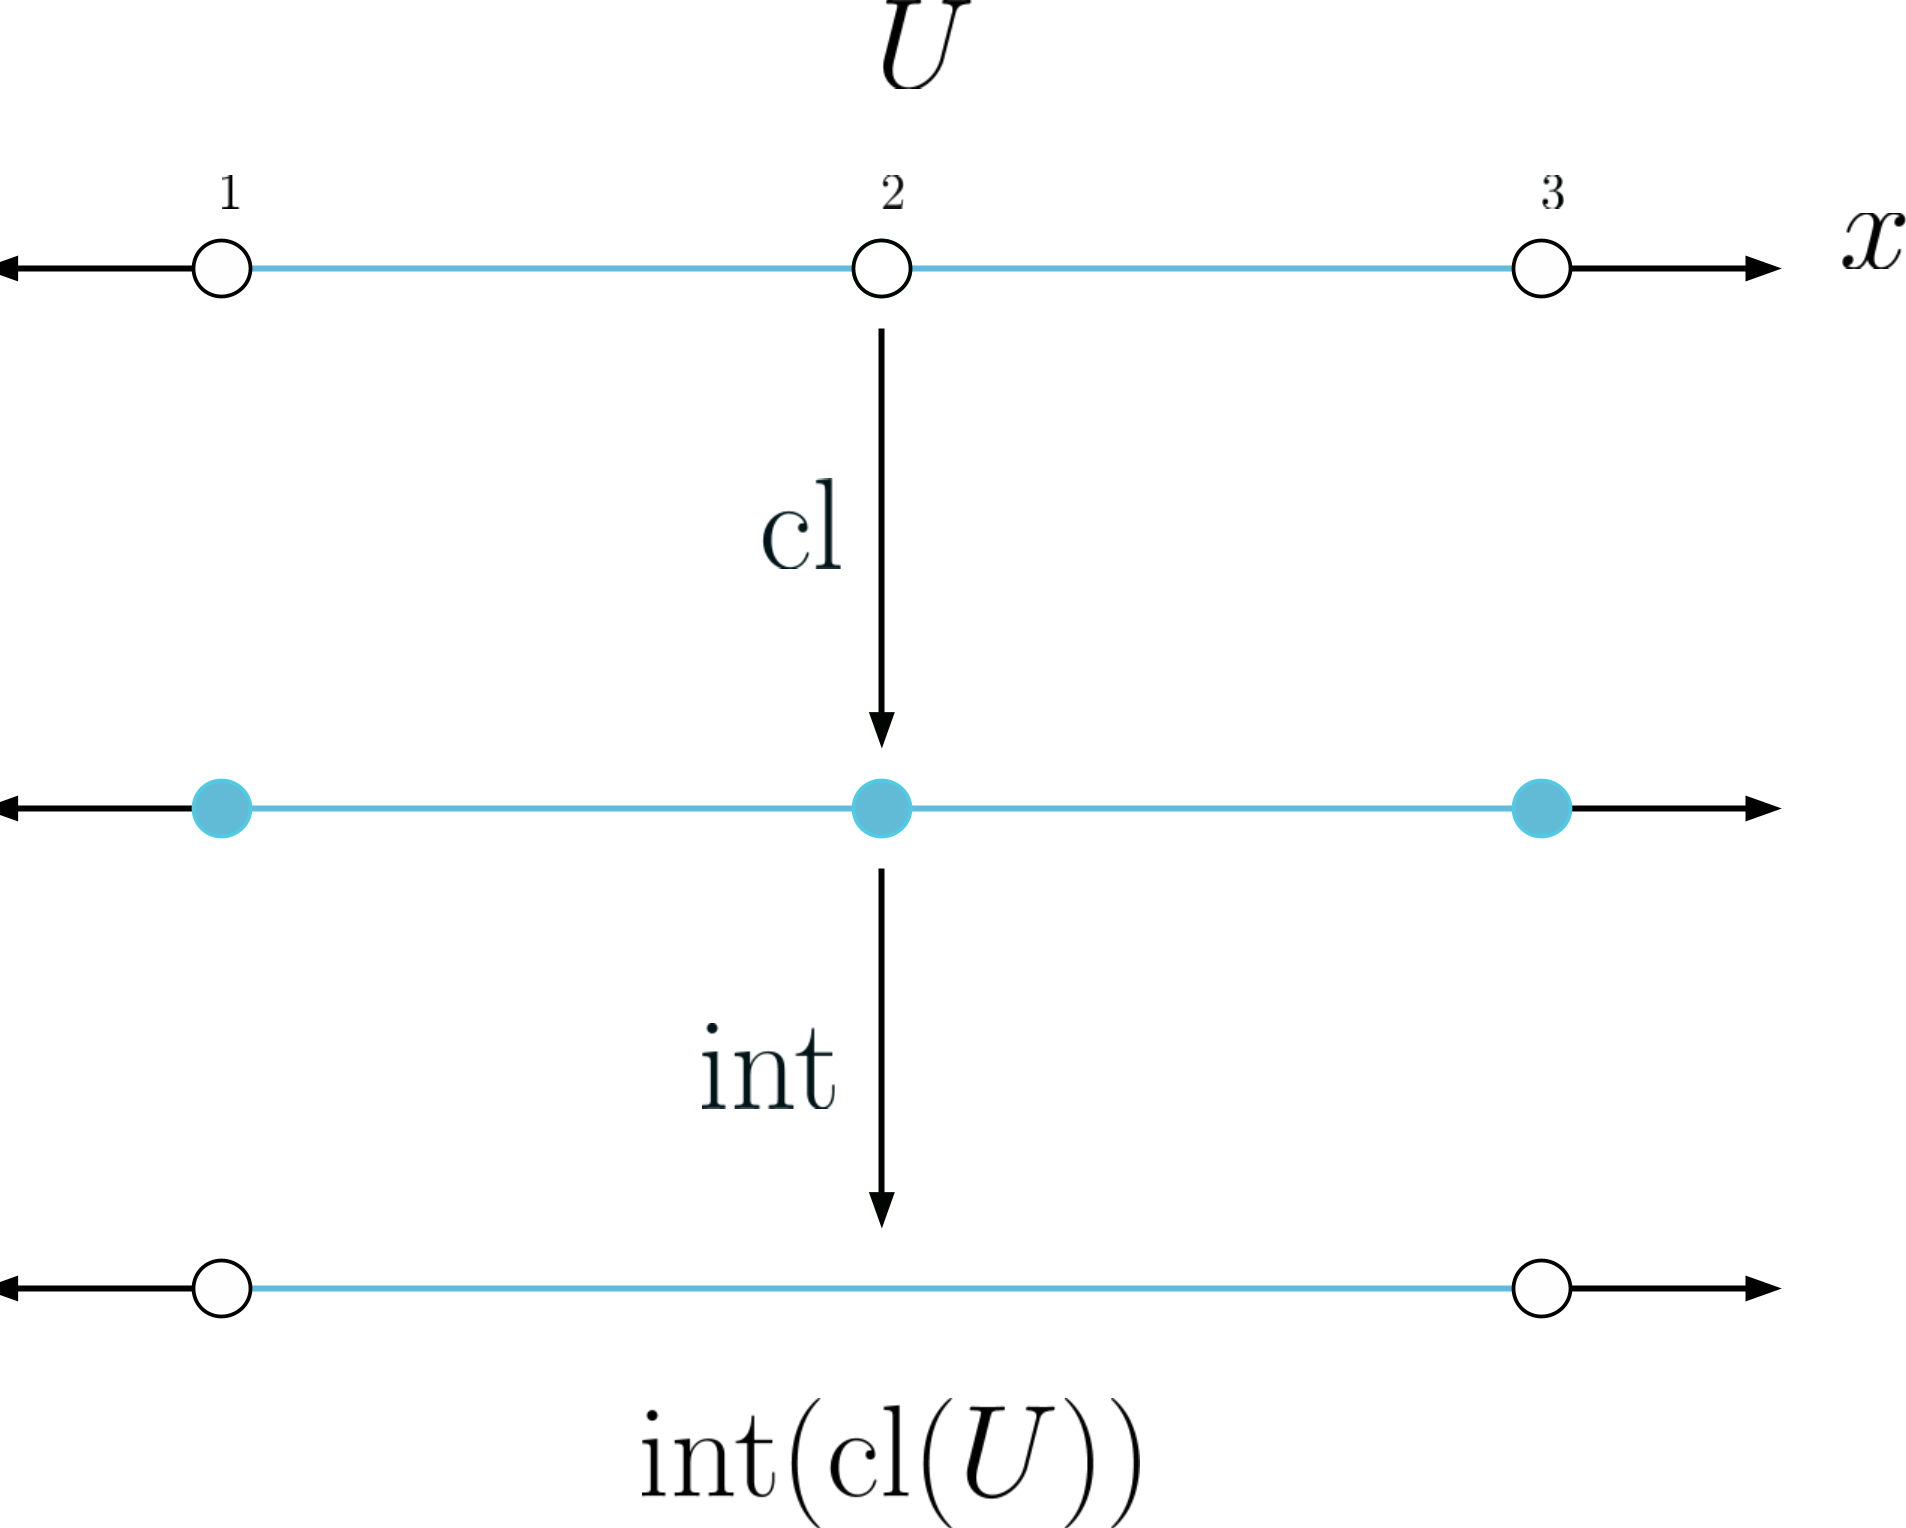
\includegraphics[scale=0.13]{e2fig3.png}
	\caption{El conjunto $U$ es abierto en la topología usual sobre $\mathbb{R}$, pero no abierto regular. }
\end{figure}

Notamos que la frontera de $U$ es $\{ 1, 2, 3 \}$, de modo que cuando se toma la clausura, se agregan estos tres puntos. Al tomar el interior, nos deshacemos de los puntos $1$ y $3$: ningún entorno de estos puntos está contenido en $\text{cl}(U)$. Sin embargo, notamos que $2$ \textit{está rodeado} de elementos de $U$ sin pertenecer a $U$: existe un entorno de $2$ que, aparte del mismo punto $2$, solo contiene elementos de $U$. De forma equivalente, existe un entorno $V$ de $2$ tal que $( V \backslash \{ 2 \} )\cap (X \backslash U) = \varnothing$. \\

\textbf{Proposición. } Sea $X$ un espacio topológico y $U \subseteq X$ abierto. Si existe un $x \in \partial U$ y un entorno $V$ de $x$ tal que $(V \backslash \{x\}) \cap (X \backslash U) = \varnothing$, entonces $U$ no es abierto regular. 
\begin{proof}
	Mostramos que $x \notin U$ y $x \in \text{int}(\text{cl}(U))$. Al ser un conjunto abierto, se sigue que $U$ y $\partial U$ son disjuntos, de forma que $x \notin U$. Puesto que $\text{cl}(U) = \text{int}(U) \cup \partial U$, se sigue que $x \in \text{cl}(U)$. Ahora mostraremos que $x$ está en el interior de este último conjunto. Notemos que la hipótesis nos dice que hay un entorno $V$ de $x$ tal que $(V \backslash \{x\}) \cap (X \backslash U) = \varnothing$. De esto, podemos deducir que
	$$ V \subseteq U \cup \{ x \} \subseteq \text{cl}(U). $$
	De forma que existe un entorno de $x$ contenido en $\text{cl}(U)$. Por tanto, $x$ está en  $\text{int}(\text{cl}(U))$.
\end{proof}

\end{document}
